\documentclass[class=article,11pt,border=6pt]{standalone}
% Standalone build of Figure 1 of "The Router Already Knows".
% The picture code is copied verbatim from the paper's source.
\usepackage[T1]{fontenc}
\usepackage[sc]{mathpazo}
\linespread{1.045}
\usepackage{amsmath,amssymb}
\usepackage{xcolor}
\usepackage{tikz}
\usetikzlibrary{arrows.meta,calc}
\begin{document}
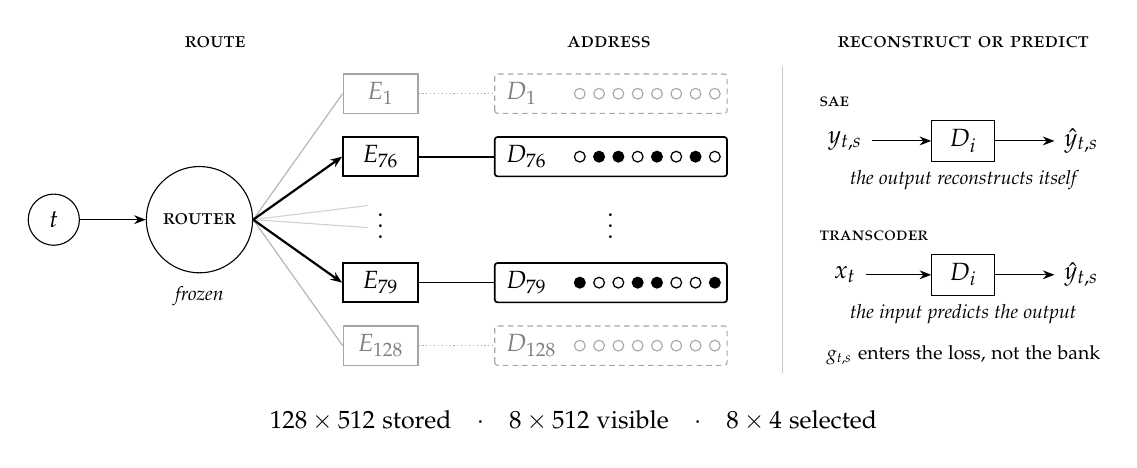
\begin{tikzpicture}[
  font=\small,
  >={Stealth[length=4.2pt,width=3.2pt]},
  exp/.style={draw, minimum width=9.5mm, minimum height=5mm, inner sep=1pt},
]
\node[font=\footnotesize\scshape] at (2.05,2.25) {route};
\node[font=\footnotesize\scshape] at (7.05,2.25) {address};
\node[font=\footnotesize\scshape] at (11.55,2.25) {reconstruct or predict};
\node[circle, draw, minimum size=6.5mm, inner sep=0pt] (t) at (0,0) {$t$};
\node[circle, draw, minimum size=13.5mm, inner sep=0pt, font=\footnotesize\scshape] (r) at (1.85,0) {router};
\node[font=\scriptsize\itshape, anchor=north] at (1.85,-0.72) {frozen};
\draw[->] (t) -- (r);
\node[exp, draw=black!35, text=black!50] (e1)   at (4.15, 1.6) {$E_{1}$};
\node[exp, line width=0.8pt]            (e37)  at (4.15, 0.8) {$E_{76}$};
\node                                    (ed)   at (4.15, 0.02) {$\vdots$};
\node[exp, line width=0.8pt]            (e94)  at (4.15,-0.8) {$E_{79}$};
\node[exp, draw=black!35, text=black!50] (e128) at (4.15,-1.6) {$E_{128}$};
\draw[black!30] (r.east) -- (e1.west);
\draw[black!30] (r.east) -- (e128.west);
\draw[black!18] (r.east) -- ($(ed.west)+(0,0.16)$);
\draw[black!18] (r.east) -- ($(ed.west)+(0,-0.12)$);
\draw[->, line width=0.8pt] (r.east) -- (e37.west);
\draw[->, line width=0.8pt] (r.east) -- (e94.west);
\newcommand{\bank}[4]{%
  \ifnum#3=1
    \draw[rounded corners=1pt, line width=0.6pt] (5.6,#1-0.25) rectangle (8.55,#1+0.25);
    \node[anchor=west] at (5.62,#1) {$D_{#2}$};
    \foreach \k in {0,...,7} {\draw[line width=0.45pt] (6.68+\k*0.245,#1) circle (0.068);}
    \foreach \k in {#4} {\fill (6.68+\k*0.245,#1) circle (0.068);}
  \else
    \draw[rounded corners=1pt, black!35, dash pattern=on 2pt off 1.5pt] (5.6,#1-0.25) rectangle (8.55,#1+0.25);
    \node[anchor=west, black!50] at (5.62,#1) {$D_{#2}$};
    \foreach \k in {0,...,7} {\draw[black!35, line width=0.4pt] (6.68+\k*0.245,#1) circle (0.068);}
  \fi}
\bank{1.6}{1}{0}{}
\bank{0.8}{76}{1}{1,2,4,6}
\node at (7.07,0.02) {$\vdots$};
\bank{-0.8}{79}{1}{0,3,4,7}
\bank{-1.6}{128}{0}{}
\draw[black!35, densely dotted] (e1.east) -- (5.6,1.6);
\draw[black!35, densely dotted] (e128.east) -- (5.6,-1.6);
\draw[line width=0.6pt] (e37.east) -- (5.6,0.8);
\draw[line width=0.6pt] (e94.east) -- (5.6,-0.8);
\draw[black!22] (9.25,-1.95) -- (9.25,1.95);
\node[font=\scriptsize\scshape, anchor=west] at (9.6,1.5) {sae};
\node (ys)  at (10.05,1.0) {$y_{t,s}$};
\node[draw, minimum width=8mm, minimum height=5mm] (ds) at (11.55,1.0) {$D_i$};
\node (yh1) at (13.05,1.0) {$\hat y_{t,s}$};
\draw[->] (ys) -- (ds); \draw[->] (ds) -- (yh1);
\node[font=\scriptsize\itshape] at (11.55,0.5) {the output reconstructs itself};
\node[font=\scriptsize\scshape, anchor=west] at (9.6,-0.2) {transcoder};
\node (xt)  at (10.05,-0.7) {$x_{t}$};
\node[draw, minimum width=8mm, minimum height=5mm] (dt) at (11.55,-0.7) {$D_i$};
\node (yh2) at (13.05,-0.7) {$\hat y_{t,s}$};
\draw[->] (xt) -- (dt); \draw[->] (dt) -- (yh2);
\node[font=\scriptsize\itshape] at (11.55,-1.2) {the input predicts the output};
\node[font=\scriptsize] at (11.55,-1.72) {$g_{t,s}$ enters the loss, not the bank};
\node[font=\small] at (6.6,-2.55) {$128\times512$ stored\quad$\cdot$\quad$8\times512$ visible\quad$\cdot$\quad$8\times4$ selected};
\end{tikzpicture}
\end{document}
